\documentclass[a4paper]{article}

\usepackage[utf8]{inputenc}
\usepackage[14pt]{extsizes}
\usepackage[english,russian]{babel}
\usepackage{graphicx}
\usepackage[left=20mm, top=15mm, right=15mm, bottom=15mm, nohead, footskip=10mm]{geometry} 
 
\begin{document}

\begin{center}
 Гафни Даниил, 406 группа\\
 \textit{Постановка задачи}
\end{center}

Импульсные (спайковые) нейронные сети (СНС) являются перспективным нейроморфным алгоритмом, биологически корректно моделируя взаимодействия нейронов мозга. Наибольший интерес СНС представляют для решения задач в реальном времени (принятие решений, распознавание образов), так как могут быть реализованы на специализированном вычислительно- и энергоэффективном мемристорном нейрочипе. В отличие от формальных нейронных сетей, в спайковых сетях нейроны обмениваются дискретными электрическими сигналами (спайками), существующими во времени. При накоплении потенциала, превышающего определенный порог активации, нейрон сам испускает спайк. Влияние входящих спайков на потенциал нейрона определяется значением веса межнейронной связи.

Стандартные методы обучения весов связей, применяющиеся в формальных нейронных сетях (метод обратного распространения ошибки) не представляется возможным применять к СНС из-за их дискретной и распределенной во времени природы. Таким образом, исследование алгоритмов обучения СНС представляется важной задачей.

В этой работе будет исследовано влияение конкуренции между нейронами с общим рецептивным полем на точность распознавания изображения для LSCNN архитектуры.

\begin{figure}[b!]
 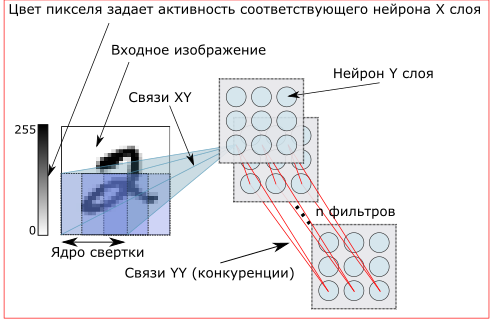
\includegraphics{LCSNN.png}
 \caption{Архитектура LCSNN}
 \label{Изображение 1: Архитектура LCSNN}
\end{figure}


\end{document}
